% 编译：xelatex report.tex（两遍），或 tectonic report.tex；Overleaf 上选择 XeLaTeX。
\documentclass[UTF8,11pt,a4paper]{ctexart}
\usepackage[margin=2.2cm]{geometry}
\usepackage{amsmath,amssymb}
\usepackage{booktabs}
\usepackage{graphicx}
\usepackage{enumitem}
\usepackage{caption}
\usepackage{float}
\usepackage[hidelinks]{hyperref}
\setlist{nosep,leftmargin=1.6em}
\captionsetup{font=small,labelfont=bf,skip=4pt}
\setlength{\textfloatsep}{8pt}\setlength{\intextsep}{8pt}
\graphicspath{{figures/}}

\title{第一类环境（代际与养老金）rule-based 版\\ \large 环境设定与运行结果}
\author{}
\date{2026 年 10 月 10 日}

\begin{document}
\maketitle

\section{概述}

\begin{itemize}
  \item 按设计文档第一类的世界规则实现了一个可运行的环境。所有角色按固定规则行动，没有强化学习和动态规划。
  \item 代码在 \texttt{olg\_pension\_env/}，分层仿照 EconGym（配置、世界规则、环境核心、决策规则、运行器、验证），全部自写。
  \item 两项验证通过：五条会计恒等式的残差为 $10^{-15}$ 量级；人口回声的周期与衰减率和理论值相差不到 0.3\%。
  \item 运行结果（\texttt{aging} 场景）见第 6 节的两张图：缴费率出现约 135 年的长周期，基金在第 156 年耗尽，此后 24 年待遇被削减。
\end{itemize}

\section{环境设定}

\subsection{时间结构}

一步为一年，主运行 $T=200$ 年。三个时钟：生产率冲击每年一次（快）；政策每 $H=5$ 年调整一次（中）；人口结构由分年龄进入率与存活率驱动（慢）。每年的执行顺序：
\begin{enumerate}
  \item 人口更新；上一年的储蓄由存活者带入，死者的部分留作遗产。
  \item 生产率冲击实现。
  \item 若 $t \bmod H = 0$，养老金当局调整政策。
  \item 由资本和劳动得到利率与工资；结算基金，必要时触发自动平衡。
  \item 家庭选择储蓄比例，得到消费与下一年资产。
  \item 更新各类型的预期；计算奖励；核对会计恒等式。
\end{enumerate}
劳动无弹性，因此第 4 步不需要期内迭代。

\subsection{人口}

模型年龄 $j=1,\dots,80$ 对应真实年龄 21 至 100 岁，$N_{j,t}$ 为队列人数：
\begin{equation}
  N_{j+1,t+1} = \psi_{j+1}\,N_{j,t}, \qquad N_{1,t+1} = \sum_{j} f_j\,N_{j,t}.
\end{equation}
$\psi_j$ 为条件存活率。$f_j$ 为进入率：年龄 $j$ 的每个人在下一年带来的 21 岁新进入者数。父母在真实年龄 20--45 岁生育，孩子 21 年后进入，所以 $f_j$ 在模型年龄 21--46 为正、均值 31。$f$ 的水平按 Leslie 矩阵主特征值 $\lambda$ 缩放，$\lambda=1$ 为平稳人口。

\subsection{生产与价格}

\begin{align}
  Y_t &= Z_t K_t^{\alpha} L_t^{1-\alpha}, & \log Z_t &= g\,t + z_t, & z_t &= \rho_z z_{t-1} + \sigma_z \varepsilon_t,\\
  r_t &= \alpha Y_t/K_t - \delta, & w_t &= (1-\alpha) Y_t/L_t. & &
\end{align}
资本 $K_t$ 等于上一年的全部私人储蓄（含当年死者的部分）加养老基金 $F_t$；劳动 $L_t=\sum_{j<J_R} N_{j,t}\,e_j\,\bar\ell$，$e_j$ 为年龄效率，$\bar\ell=1/3$。G1 配置下没有财政当局，劳动税、国债、政府支出均为零。

\subsection{家庭}

一个家庭是“出生队列 $\times$ 行为类型”的代表性个体。可支配资源、消费与储蓄为
\begin{align}
  x_{j,t} &= (1+r_t)\,a_{j,t} + (1-\tau_{p,t})\,w_t e_j \bar\ell\;\mathbf{1}[j<J_R] + b_t\,\mathbf{1}[j\ge J_R] + tr_t,\\
  c_{j,t} &= (1-s_{j,t})\,x_{j,t}, \qquad a_{j+1,t+1} = s_{j,t}\,x_{j,t}, \qquad s\in[0,\,0.99].
\end{align}
$tr_t$ 为意外遗产：死者的储蓄连同当年利息平均分给全部在世者。新进入者资产为零。效用为 $u = c^{1-\sigma}/(1-\sigma) - \chi\,\ell^{1+1/\varphi}/(1+1/\varphi)$。

\subsection{养老金当局}

带结余基金的现收现付制。记 $\bar w_t = w_t L_t / N^W_t$ 为在职者平均工资，$N^W_t$、$N^R_t$ 为在职与退休人数：
\begin{equation}
  b_t = \kappa_t\,\bar w_t, \qquad F_{t+1} = (1+r_t)F_t + \tau_{p,t}\,w_t L_t - b_t N^R_t .
\end{equation}
\textbf{自动平衡}：若上式给出 $F_{t+1}<0$，当年待遇削减为 $b_t = [(1+r_t)F_t + \tau_{p,t} w_t L_t]/N^R_t$，使 $F_{t+1}=0$，记一次触发，回合不终止。政策工具见表~\ref{tab:policy}。

\begin{table}[H]
\centering\small
\caption{政策工具与约束}\label{tab:policy}
\begin{tabular}{lccc}
\toprule
工具 & 取值范围 & 每次最大调整 & 初值 \\
\midrule
缴费率 $\tau_p$ & $[0,\,0.4]$ & $0.02$ & $0.14$ \\
替代率 $\kappa$ & $[0,\,1]$ & $0.05$ & $0.40$ \\
退休年龄 $J_R$ & $60$--$70$ & $1$ 岁 & $65$ \\
\bottomrule
\end{tabular}
\end{table}

初始人口下收支恰好平衡的缴费率为 $\kappa\cdot DR = 0.40\times 0.39 = 0.156$，其中 $DR=N^R/N^W$ 为抚养比。默认的 0.14 略欠筹资。

\subsection{奖励、回合与初始状态}

家庭的奖励为当年效用。养老金当局的奖励为 $W_t - \phi_F\,\mathbf{1}[\text{触发}]$，$W_t$ 为在世者效用的人口加权平均。回合长度固定为 200 年。初始状态分两步得到。年龄结构取给定增长率下的稳定分布，由存活率直接算出。各年龄的资产则由燃烧期确定：从人人资产相同出发，在政策固定、冲击关闭、基金占产出比冻结在 0.5 的条件下运行，直到 $K/Y$ 收敛（100--190 年），再把水平变量缩回 $Z=1$ 的尺度；燃烧期的数据不计入结果。

\section{决策规则}

\subsection{家庭}

把一生资源平摊到期望剩余寿命：
\begin{equation}\label{eq:rule}
  c_{j,k,t} = \theta\;\frac{x_{j,k,t} + PV^{w}_{j,t} + \kappa^{e}_{j,k,t}\,\bar w_t\, H^{p}_{j,t}}{H_{j}}, \qquad c_{j,k,t} \le x_{j,k,t} ,\qquad s_{j,k,t} = 1 - c_{j,k,t}/x_{j,k,t} .
\end{equation}
$j$ 为年龄，$k$ 为行为类型，$t$ 为年份；$\theta=1.132$ 由校准得到。记 $\Psi_{j,m}=\prod_{i=j+1}^{m}\psi_i$ 为 $j$ 岁的人活到 $m$ 岁的概率（$\Psi_{j,j}=1$），$J=80$ 为最高年龄，则
\begin{align}
  H_{j} &= \sum_{m=j}^{J}\Psi_{j,m}, && \text{期望剩余寿命，含当年；}\\
  PV^{w}_{j,t} &= \sum_{m=j+1}^{J_{R,t}-1}\Psi_{j,m}\,(1-\tau_{p,t})\,w_t\,e_m\,\bar\ell, && \text{明年起到退休前的税后工资之和；}\\
  H^{p}_{j,t} &= \sum_{m=\max(j+1,\,J_{R,t})}^{J}\Psi_{j,m}, && \text{明年起领取养老金的期望年数。}
\end{align}
后两项从明年算起，因为当年的工资或养老金已包含在 $x_{j,k,t}$ 中。$\kappa^e_{j,k,t}$ 是家庭对自己退休后替代率的预期，是式中唯一依赖家庭对政策看法的量：预期越低，消费越少，储蓄越多。

式~\eqref{eq:rule} 每年对每个年龄、每种类型重新计算。家庭不知道未来的价格与政策：上式中的 $w_t$、$\tau_{p,t}$、$J_{R,t}$ 都取当年的值，并假设此后不变；存活概率 $\psi$ 与年龄效率 $e$ 是固定的已知表。类型之间的差别来自两处：$\kappa^e_{j,k,t}$ 不同，以及由过去的储蓄累积而成的 $x_{j,k,t}$ 不同。

四种行为类型共用式~\eqref{eq:rule}，区别见表~\ref{tab:types}。每个队列带着自己的 $\kappa^e$ 逐年老化，进入时 $\kappa^e=\kappa_t$。

A、S 型根据一个“信号” $\kappa^{sig}_t$ 修正预期，即他们认为制度实际能兑现的替代率。记 $\kappa^{real}_t=b_t/\bar w_t$ 为当年实际兑现的替代率。$\tau_{p,t}/DR_t$ 是不动用基金、只把当年缴费平分给退休者时能发的替代率。信号按一条警戒线取值：
\begin{equation}\label{eq:signal}
  \kappa^{sig}_t =
  \begin{cases}
    \kappa^{real}_t, & F_{t+1}/Y_t \ge 0.5,\\[2pt]
    \min\!\left(\kappa^{real}_t,\ \tau_{p,t}/DR_t\right), & F_{t+1}/Y_t < 0.5.
  \end{cases}
\end{equation}
即基金占产出比不低于 $0.5$（初始水平）时相信实际发放；低于这条线时不再相信承诺，改按当年缴费够发多少来预期。因此 A、S 型在待遇被削减之前，就会因基金下降而下调预期。

\begin{table}[H]
\centering\small
\caption{四种行为类型}\label{tab:types}
\begin{tabular}{llp{4.6cm}}
\toprule
类型 & 预期的更新 & 其他修正 \\
\midrule
R 理性基准 & $\kappa^{e\prime} = \kappa$ & 无 \\
P 现时偏好 & $\kappa^{e\prime} = \kappa$ & $c$ 乘以 $1.15$ \\
A 学习型 & $\kappa^{e\prime} = \kappa^{e} + 0.05\,(\kappa^{sig} - \kappa^{e})$ & 无 \\
S 社会型 & $\kappa^{e\prime} = 0.7\,[\text{A 型更新}] + 0.3\,\overline{\kappa^{e}}_{\text{同龄}}$ & $s_{j,t} = 0.7\,s^{\text{规则}}_{j,t} + 0.3\,\bar s_{j,t-1}$ \\
\bottomrule
\end{tabular}
\end{table}

同龄平均指同一年龄内各类型按占比加权。$s^{\text{规则}}_{j,t}$ 是式~\eqref{eq:rule} 给出的储蓄比例；$\bar s_{j,t-1}$ 是上一年处在年龄 $j$ 的各类型实际储蓄比例的平均。家庭决策时别人当年的选择尚未发生，所以 S 型参照的是上一年的值；燃烧期第一年没有上一年，S 型不做混合。

另有一条只用于对账的简化规则：在职者固定 $s=0.691$，退休者 $c=x/H_j$。

\subsection{养老金当局}

两种规则：(i) 固定，沿用初始政策；(ii) 基金占比规则，决策年份若 $F/Y<0.2$ 则 $\tau_p$ 上调 $0.02$，若 $F/Y>2.0$ 则下调 $0.02$，$\kappa$ 与 $J_R$ 不动。

\section{参数与数据}

\begin{table}[H]
\centering\small
\caption{参数}\label{tab:params}
\begin{tabular}{lll}
\toprule
参数 & 取值 & 来源 \\
\midrule
$\alpha,\ \delta,\ g$ & $0.33,\ 0.06,\ 0.015$ & 设计文档 \\
$\rho_z,\ \sigma_z$ & $0.9,\ 0.02$ & 设计文档 \\
$\sigma,\ \varphi,\ \chi$ & $2,\ 0.5,\ 1$ & 设计文档；$\chi$ 为设定 \\
存活率 $\psi_j$ & 路径 & 美国 CDC 2022 死亡率，插值到单岁 \\
进入率 $f_j$ & 钟形，均值 31、标准差 5 & 人造；水平按 $\lambda$ 缩放 \\
年龄效率 $e_j$ & 二次式，48 岁见顶 & 美国 SCF 2022 工资对年龄回归 \\
$\theta$ & $1.132$ & 校准：燃烧期 $K/Y=3$（R 型）\\
固定储蓄比例 & $0.691$ & 校准：燃烧期 $K/Y=3$ \\
P 加码、A 增益、S 权重 & $0.15,\ 0.05,\ 0.3$ & 设定，未校准 \\
A、S 型的基金警戒线 & $0.5$ & 设定：等于初始基金占产出比 \\
$\phi_F,\ \beta$ & $1,\ 0.96$ & 设定 \\
\bottomrule
\end{tabular}
\end{table}

设计文档用贴现因子匹配 $K/Y\approx 3$；rule-based 没有贴现因子，改为对储蓄规则的参数做二分。

\section{验证}

\paragraph{会计恒等式} 每年核对以下五条，残差相对 GDP 超过 $10^{-8}$ 即报错。五个场景各 200 年的最大残差不超过 $2\times10^{-15}$，含政策调整与自动平衡的场景同样通过。
\begin{center}\small
\begin{tabular}{ll}
\toprule
商品市场 & $K_{t+1} = (1-\delta)K_t + Y_t - C_t$ \\
基金收支 & $F_{t+1} = (1+r_t)F_t + \text{缴费} - \text{待遇}$ \\
家庭预算 & $\sum N(c+a') = \sum N x$ \\
遗产分配 & $tr_t\,N_t = (1+r_t)\times\text{死者资产}$ \\
资产守恒 & 上年总储蓄 $=$ 死者资产 $+$ 存活者带入资产 \\
\bottomrule
\end{tabular}
\end{center}

\paragraph{人口回声} 只用人口模块，给平稳人口一次性的进入冲击，与 Leslie 矩阵第二特征值 $\lambda_2 = 0.966 \pm 0.196\,i$ 的理论值比较（表~\ref{tab:echo}）。主特征值为 1，所以一次性多进入的人会永久抬高人口水平，回声是围绕新水平的振荡；量衰减时先减去长期水平，并从第二次回声开始量。冲击为 $+50\%$ 时，新进入人数长期高出 $1.6\%$，在此之上各次回声的幅度依次约为 $2.5\%$、$1.3\%$、$0.8\%$、$0.5\%$（第 32、63、94、125 年）。

\begin{table}[H]
\centering\small
\caption{人口回声检验}\label{tab:echo}
\begin{tabular}{lccc}
\toprule
 & 理论值 & 模拟值 & 相对误差 \\
\midrule
周期 $2\pi/|\arg\lambda_2|$（年） & $31.31$ & $31.20$ & $0.3\%$ \\
每年衰减 $|\lambda_2|$ & $0.9854$ & $0.9851$ & $0.03\%$ \\
每次回声相对上一次 & $0.630$ & $0.626$ & $0.6\%$ \\
\bottomrule
\end{tabular}
\end{table}

\paragraph{增长率} 模拟的产出增长率为 $2.28\%$，平衡增长的理论值为 $g/(1-\alpha)=2.24\%$；人口每年收缩 $0.5\%$ 的场景为 $1.74\%$，与 $2.24\%-0.5\%$ 一致。

设计文档中其余检验（Diamond 挤出、Samuelson--Aaron、现时偏好、RL 家庭精度）需要优化型家庭，本阶段未做。

\section{运行结果：\texttt{aging} 场景}

\paragraph{基本设定} 单一随机种子，运行 200 年。
\begin{itemize}
  \item \textbf{人口}：每年收缩 $0.5\%$（$\lambda=0.995$），抚养比约 $0.46$；第 10 年新进入的队列多 $30\%$。
  \item \textbf{政策}：缴费率初值 $0.14$，替代率 $0.40$，退休年龄 65。每 5 年检查一次基金占产出比，低于 $0.2$ 则缴费率加 $0.02$，高于 $2.0$ 则减 $0.02$，否则不动；替代率与退休年龄不调整。
  \item \textbf{家庭}：按式~\eqref{eq:rule} 决定储蓄；R/P/A/S 四种类型占比 $0.4/0.2/0.2/0.2$。
  \item \textbf{其余参数}：见表~\ref{tab:params}。
\end{itemize}

\begin{figure}[H]
\centering
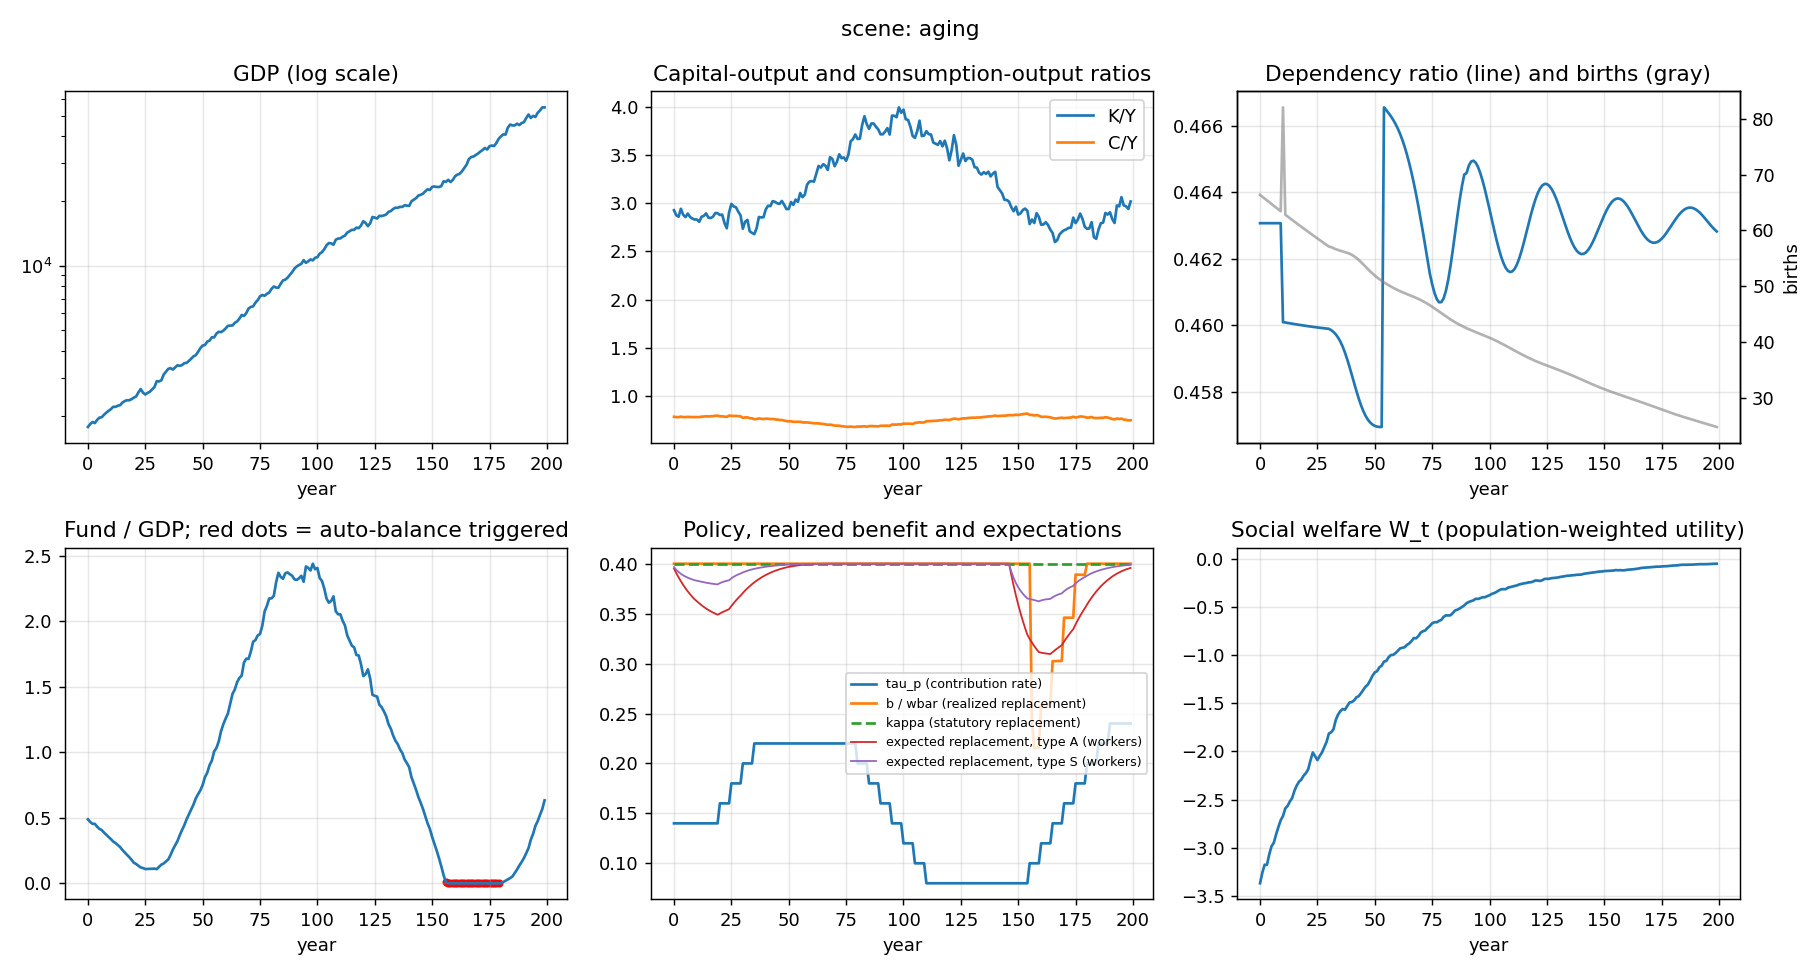
\includegraphics[width=\textwidth]{aging_overview.png}
\caption{总量路径。上排：产出（对数刻度）；资本产出比与消费产出比；抚养比（蓝）与每年新进入人数（灰）。下排：基金占产出比，红点为自动平衡触发（待遇被削减）的年份；缴费率、规则替代率、实际替代率，以及 A、S 型在职者的平均预期替代率；社会福利。}\label{fig:aging}
\end{figure}

\begin{figure}[H]
\centering
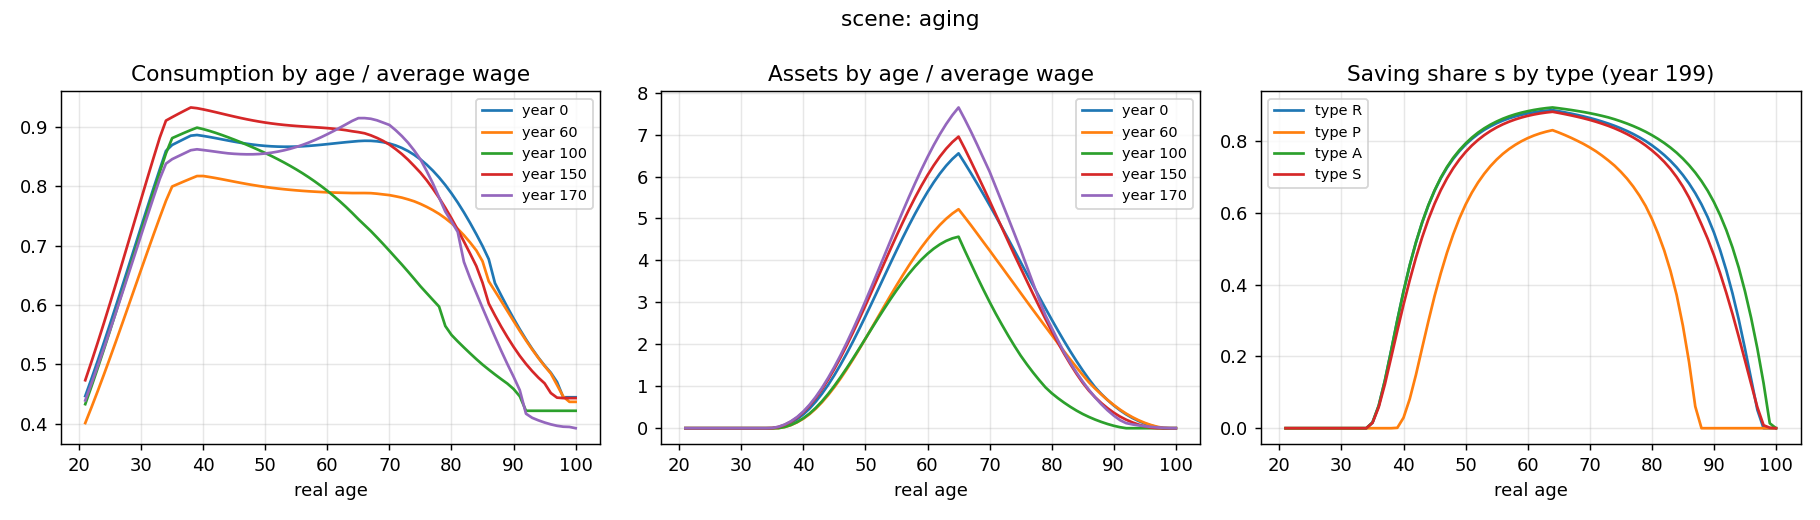
\includegraphics[width=\textwidth]{aging_cohorts.png}
\caption{分年龄剖面。左、中：五个年份的分年龄消费与资产，均除以当年的在职者平均工资；第 60、100、150、170 年分别对应高缴费、基金最高、低缴费、待遇削减。右：第 199 年各行为类型的储蓄比例。}\label{fig:aging-cohorts}
\end{figure}

\section{局限与待确认}

\begin{itemize}
  \item 只报告了 \texttt{aging} 一个场景、一个随机种子。
  \item 政策规则的阈值（$0.2$、$2.0$）与步长（$0.02$）是设定值，周期的长度取决于它们。
  \item 家庭是队列代表，同一队列同一类型内没有收入与财富差异。
  \item 三个时钟（外生冲击、政策间隔、人口方程）的周期由环境给定。图中 135 年的缴费率周期不是环境给定的，而是政策规则产生的；但它来自规则的设定，不是家庭行为的结果。
  \item 四种类型的行为参数是设定值；数据来自美国，设计文档未指定校准对象。
  \item 需确认的设定：预期按替代率而非金额形成；退休年龄上调时已退休队列回到劳动市场；自动平衡在家庭消费之前决定当年待遇；S 型的同龄人取同一年龄的全部类型，储蓄参照的是上一年的实际值。
\end{itemize}

\end{document}
